\section{Results}
While to this point insufficient progress has been made to allow rigorous
testing of the discrete maximum principle coding within a use code, test
scripts were developed that evaluate the ability of the class
\texttt{DiscreteMaxPrinciple} to test for DMP violations around
previously-performed numerical analyses.  The \texttt{DiscreteMaxPrinciple}
class implements all of the adjustments to the DMP discussed to this point in
this work into a \texttt{C++} code environment intended to be used within
\texttt{clubimc}, developed at Los Alamos National Laboratory. To test this
class, the same input parameters as in \cite{WolLarDen} were used and a
dozen
test cases were checked. Half of these tests had $\Delta_t,\Delta_x$ pairs that
were expected to narrowly violate the DMP, and the other half were expected to
just avoid violation. Figure \ref{passfail} shows the data points selected with
reference to the experimental DMP line of demarcation developed in
\cite{WolLarDen}, both as a whole and then magnified to see individual test
cases.  Each graph has axes of $\Delta_t$ on the x-axis and $\Delta_x$ on the
y-axis.
\begin{figure}[htb]
\centering
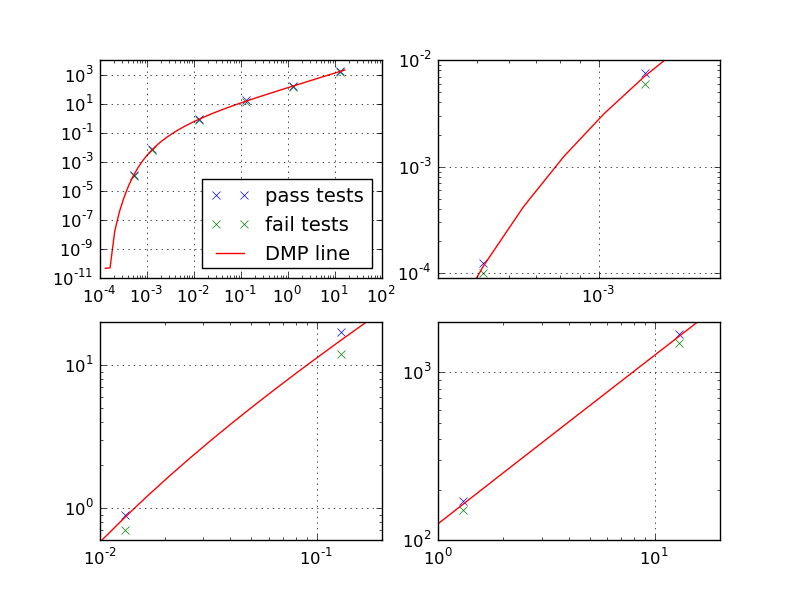
\includegraphics[width=0.9\linewidth]{pass_fail_together}
\caption{DMP Test Cases}
\label{passfail}
\end{figure}

\newpage
The table below shows the results of the test cases:
\begin{center}
\begin{tabular}{c c c c}
$\Delta_t$ & $\Delta_x$ & Expected & Calculated \\ \hline
$5.0596\times10^{-4}$ & $2.1\times10^{-4}$ & $3.74028\times10^{-6}$ &
  $3.74472\times10^{-6}$ \\
$1.6\times10^{-3}$ & $1.8\times10^{-2}$ & $3.23378\times10^{-5}$ &
  $3.23377\times10^{-5}$ \\
$1.6\times10^{-2}$ & $1.3\times10^{0}$ & $8.01371\times10^{-4}$ &
  $8.01372\times10^{-4}$ \\
$1.6\times10^{-1}$ & $1.95\times10^{1}$ & $5.69082\times10^{-3}$ &
  $5.69082\times10^{-3}$ \\
$1.6\times10^{0}$ & $2.1\times10^{2}$ & $8.31396\times10^{-2}$ &
  $8.31397\times10^{-2}$ \\
$1.6\times10^{1}$ & $2.1\times10^{3}$ & $7.33246\times10^{-1}$ &
  $7.33246\times10^{-1}$ \\ \hline
%%%%%%%%%%%%%%%%%%%%%%%%%%%%should violate v, should not ^
$5.0596\times10^{-4}$ & $1.9\times10^{-4}$ & $-5.36018\times10^{-6}$ &
  $-5.35573\times10^{-6}$ \\
$1.6\times10^{-3}$ & $1.6\times10^{-2}$ & $-3.94675\times10^{-5}$ &
  $-3.94676\times10^{-5}$ \\
$1.6\times10^{-2}$ & $1.1\times10^{0}$ & $-1.29592\times10^{-3}$ &
  $-1.29592\times10^{-3}$ \\
$1.6\times10^{-1}$ & $1.8\times10^{1}$ & $-6.81044\times10^{-3}$ &
  $-6.81043\times10^{-3}$ \\
$1.6\times10^{0}$ & $1.9\times10^{2}$ & $-7.71581\times10^{-2}$ &
  $-7.71580\times10^{-2}$ \\
$1.6\times10^{1}$ & $1.9\times10^{3}$ & $-8.60397\times10^{-1}$ &
  $-8.60396\times10^{-1}$ 
\end{tabular}
\end{center}
In the table the above, time is in shakes, distance in centimeters, and the
expected and calculated inequalities represent the value of Eq.\ \eqref{FINAL
dmp} if the $\Delta_t$ is subtracted to the right side; that is, values less
than zero violate the DMP, while those greater than zero do not.  The expected
results are from the numerical tool used in \cite{WolLarDen}, adjusted
slightly to perform multigroup calculations, and the calculated results were
obtained using the \texttt{DiscreteMaxPrinciple} class.

As can be seen, the results obtained agree very readily with the results
obtained in \cite{WolLarDen} and show, at least to a first degree, some
accuracy in this application of the discrete maximum principle to the
implicit Monte Carlo equations.